\documentclass[tikz,border=2pt]{standalone}
\usetikzlibrary{calc}
\usetikzlibrary{intersections}
\usepackage{bm}

\begin{document}

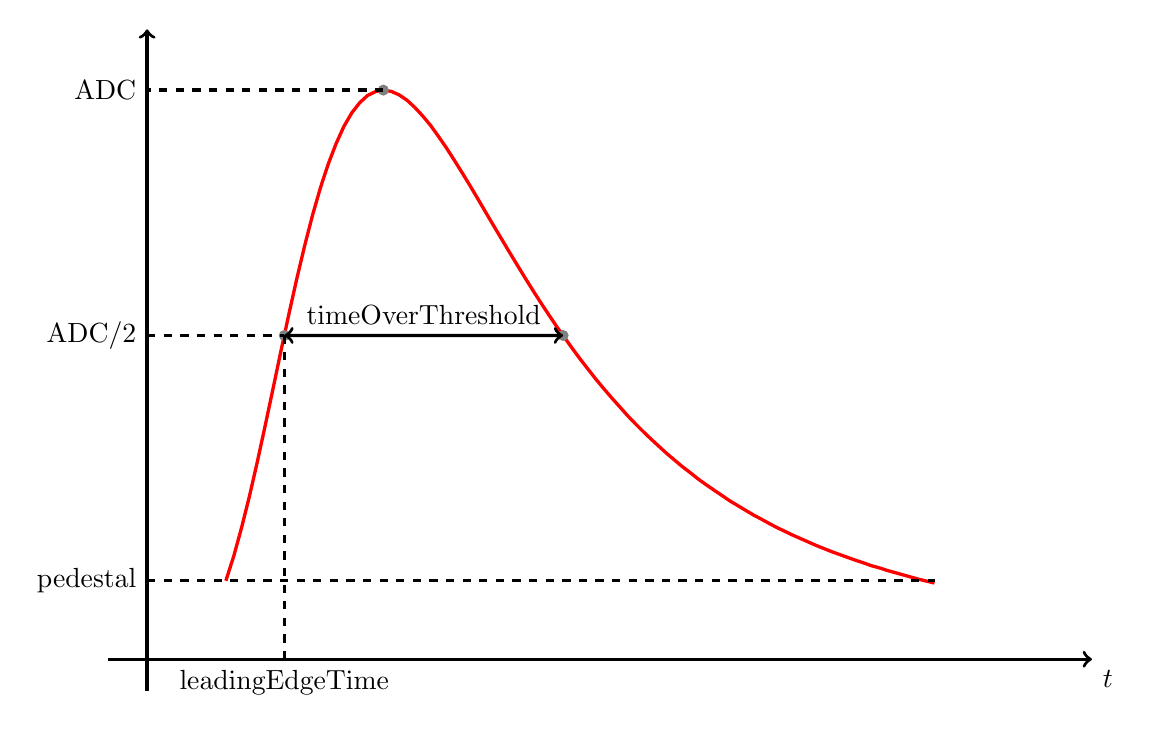
\begin{tikzpicture}[y=40cm, very thick, scale=1]
    \draw[->] (-0.5,0) -- (12, 0);
    \draw[->] (0,-0.01) -- (0,0.2);
    \node[below right] at (12,0) {$t$};
    %\node[above left] at (0,0.2) {ADC};
    
    % Landau with mu = 3, sigma = 1 
    % CLHEP/GenericFunctions/Landau.hh
    % s_max is at ( 3.0000,0.1807)
    % baseline is at ( 1.0000,0.0249)
    % (s_max - baseline)/2 + baseline = 0.1028
    \draw[name path = landau, red] 
    ( 1.0000,0.0249) -- ( 1.1000,0.0327) -- ( 1.2000,0.0418) -- ( 1.3000,0.0518) -- ( 1.4000,0.0627) -- ( 1.5000,0.0742) -- ( 1.6000,0.0860) -- ( 1.7000,0.0979) -- ( 1.8000,0.1095) -- ( 1.9000,0.1207) -- ( 2.0000,0.1312) -- ( 2.1000,0.1409) -- ( 2.2000,0.1496) -- ( 2.3000,0.1572) -- ( 2.4000,0.1637) -- ( 2.5000,0.1692) -- ( 2.6000,0.1735) -- ( 2.7000,0.1767) -- ( 2.8000,0.1790) -- ( 2.9000,0.1802) -- ( 3.0000,0.1807) -- ( 3.1000,0.1803) -- ( 3.2000,0.1792) -- ( 3.3000,0.1775) -- ( 3.4000,0.1752) -- ( 3.5000,0.1725) -- ( 3.6000,0.1695) -- ( 3.7000,0.1660) -- ( 3.8000,0.1624) -- ( 3.9000,0.1585) -- ( 4.0000,0.1545) -- ( 4.1000,0.1504) -- ( 4.2000,0.1462) -- ( 4.3000,0.1419) -- ( 4.4000,0.1377) -- ( 4.5000,0.1335) -- ( 4.6000,0.1293) -- ( 4.7000,0.1252) -- ( 4.8000,0.1211) -- ( 4.9000,0.1171) -- ( 5.0000,0.1132) -- ( 5.1000,0.1094) -- ( 5.2000,0.1057) -- ( 5.3000,0.1022) -- ( 5.4000,0.0987) -- ( 5.5000,0.0953) -- ( 5.6000,0.0921) -- ( 5.7000,0.0889) -- ( 5.8000,0.0859) -- ( 5.9000,0.0830) -- ( 6.0000,0.0802) -- ( 6.1000,0.0774) -- ( 6.2000,0.0748) -- ( 6.3000,0.0723) -- ( 6.4000,0.0699) -- ( 6.5000,0.0676) -- ( 6.6000,0.0653) -- ( 6.7000,0.0632) -- ( 6.8000,0.0611) -- ( 6.9000,0.0592) -- ( 7.0000,0.0572) -- ( 7.1000,0.0554) -- ( 7.2000,0.0537) -- ( 7.3000,0.0520) -- ( 7.4000,0.0503) -- ( 7.5000,0.0488) -- ( 7.6000,0.0473) -- ( 7.7000,0.0458) -- ( 7.8000,0.0445) -- ( 7.9000,0.0431) -- ( 8.0000,0.0418) -- ( 8.1000,0.0406) -- ( 8.2000,0.0394) -- ( 8.3000,0.0383) -- ( 8.4000,0.0372) -- ( 8.5000,0.0361) -- ( 8.6000,0.0351) -- ( 8.7000,0.0341) -- ( 8.8000,0.0332) -- ( 8.9000,0.0323) -- ( 9.0000,0.0314) -- ( 9.1000,0.0306) -- ( 9.2000,0.0297) -- ( 9.3000,0.0290) -- ( 9.4000,0.0282) -- ( 9.5000,0.0275) -- ( 9.6000,0.0268) -- ( 9.7000,0.0261) -- ( 9.8000,0.0254) -- ( 9.9000,0.0248) -- (10.0000,0.0242);
    
    % baseline
    \draw [dashed] (0,0.0249) -- (10,0.0249);
    \node [left] at (0, 0.0249) {pedestal};
    % point at max amplitude
    \coordinate (S) at ( 3.0000,0.1807);
    \fill [gray] (S) circle [radius=2pt];
    \draw [dashed] (S) -- (0,0 |- S);
    \node [left] at (0,0 |- S) {ADC};
    % points at half amplitude (minus the baseline)
    \path [name path = rising] (0,0.1028) -- (3.5, 0.1028); 
    \path [name path = falling] (4,0.1028) -- (8, 0.1028); 
    \path[name intersections={of=landau and rising, by=A}];
    \path[name intersections={of=landau and falling, by=B}];
    \fill [gray] (A) circle [radius=2pt];
    \fill [gray] (B) circle [radius=2pt];
    % time over threshold
    \draw [name path = tot, <->] (A) -- (B);
    \node [above] at ($(A)!0.5!(B)$) {timeOverThreshold};
    % leading edge time
    \draw [dashed] (A |- 0,0) -- (A |- 0,0.1028);
    \node [below] at (A |- 0,0) {leadingEdgeTime};
    \node [left] at (0,0 |- A) {ADC/2};
    \draw [dashed] (0,0 |- A) -- (A);
\end{tikzpicture}


\end{document}